% Options for packages loaded elsewhere
\PassOptionsToPackage{unicode}{hyperref}
\PassOptionsToPackage{hyphens}{url}
\PassOptionsToPackage{dvipsnames,svgnames,x11names}{xcolor}
%
\documentclass[
  letterpaper,
  DIV=11,
  numbers=noendperiod]{scrreprt}

\usepackage{amsmath,amssymb}
\usepackage{iftex}
\ifPDFTeX
  \usepackage[T1]{fontenc}
  \usepackage[utf8]{inputenc}
  \usepackage{textcomp} % provide euro and other symbols
\else % if luatex or xetex
  \usepackage{unicode-math}
  \defaultfontfeatures{Scale=MatchLowercase}
  \defaultfontfeatures[\rmfamily]{Ligatures=TeX,Scale=1}
\fi
\usepackage{lmodern}
\ifPDFTeX\else  
    % xetex/luatex font selection
\fi
% Use upquote if available, for straight quotes in verbatim environments
\IfFileExists{upquote.sty}{\usepackage{upquote}}{}
\IfFileExists{microtype.sty}{% use microtype if available
  \usepackage[]{microtype}
  \UseMicrotypeSet[protrusion]{basicmath} % disable protrusion for tt fonts
}{}
\makeatletter
\@ifundefined{KOMAClassName}{% if non-KOMA class
  \IfFileExists{parskip.sty}{%
    \usepackage{parskip}
  }{% else
    \setlength{\parindent}{0pt}
    \setlength{\parskip}{6pt plus 2pt minus 1pt}}
}{% if KOMA class
  \KOMAoptions{parskip=half}}
\makeatother
\usepackage{xcolor}
\setlength{\emergencystretch}{3em} % prevent overfull lines
\setcounter{secnumdepth}{5}
% Make \paragraph and \subparagraph free-standing
\makeatletter
\ifx\paragraph\undefined\else
  \let\oldparagraph\paragraph
  \renewcommand{\paragraph}{
    \@ifstar
      \xxxParagraphStar
      \xxxParagraphNoStar
  }
  \newcommand{\xxxParagraphStar}[1]{\oldparagraph*{#1}\mbox{}}
  \newcommand{\xxxParagraphNoStar}[1]{\oldparagraph{#1}\mbox{}}
\fi
\ifx\subparagraph\undefined\else
  \let\oldsubparagraph\subparagraph
  \renewcommand{\subparagraph}{
    \@ifstar
      \xxxSubParagraphStar
      \xxxSubParagraphNoStar
  }
  \newcommand{\xxxSubParagraphStar}[1]{\oldsubparagraph*{#1}\mbox{}}
  \newcommand{\xxxSubParagraphNoStar}[1]{\oldsubparagraph{#1}\mbox{}}
\fi
\makeatother

\usepackage{color}
\usepackage{fancyvrb}
\newcommand{\VerbBar}{|}
\newcommand{\VERB}{\Verb[commandchars=\\\{\}]}
\DefineVerbatimEnvironment{Highlighting}{Verbatim}{commandchars=\\\{\}}
% Add ',fontsize=\small' for more characters per line
\usepackage{framed}
\definecolor{shadecolor}{RGB}{241,243,245}
\newenvironment{Shaded}{\begin{snugshade}}{\end{snugshade}}
\newcommand{\AlertTok}[1]{\textcolor[rgb]{0.68,0.00,0.00}{#1}}
\newcommand{\AnnotationTok}[1]{\textcolor[rgb]{0.37,0.37,0.37}{#1}}
\newcommand{\AttributeTok}[1]{\textcolor[rgb]{0.40,0.45,0.13}{#1}}
\newcommand{\BaseNTok}[1]{\textcolor[rgb]{0.68,0.00,0.00}{#1}}
\newcommand{\BuiltInTok}[1]{\textcolor[rgb]{0.00,0.23,0.31}{#1}}
\newcommand{\CharTok}[1]{\textcolor[rgb]{0.13,0.47,0.30}{#1}}
\newcommand{\CommentTok}[1]{\textcolor[rgb]{0.37,0.37,0.37}{#1}}
\newcommand{\CommentVarTok}[1]{\textcolor[rgb]{0.37,0.37,0.37}{\textit{#1}}}
\newcommand{\ConstantTok}[1]{\textcolor[rgb]{0.56,0.35,0.01}{#1}}
\newcommand{\ControlFlowTok}[1]{\textcolor[rgb]{0.00,0.23,0.31}{\textbf{#1}}}
\newcommand{\DataTypeTok}[1]{\textcolor[rgb]{0.68,0.00,0.00}{#1}}
\newcommand{\DecValTok}[1]{\textcolor[rgb]{0.68,0.00,0.00}{#1}}
\newcommand{\DocumentationTok}[1]{\textcolor[rgb]{0.37,0.37,0.37}{\textit{#1}}}
\newcommand{\ErrorTok}[1]{\textcolor[rgb]{0.68,0.00,0.00}{#1}}
\newcommand{\ExtensionTok}[1]{\textcolor[rgb]{0.00,0.23,0.31}{#1}}
\newcommand{\FloatTok}[1]{\textcolor[rgb]{0.68,0.00,0.00}{#1}}
\newcommand{\FunctionTok}[1]{\textcolor[rgb]{0.28,0.35,0.67}{#1}}
\newcommand{\ImportTok}[1]{\textcolor[rgb]{0.00,0.46,0.62}{#1}}
\newcommand{\InformationTok}[1]{\textcolor[rgb]{0.37,0.37,0.37}{#1}}
\newcommand{\KeywordTok}[1]{\textcolor[rgb]{0.00,0.23,0.31}{\textbf{#1}}}
\newcommand{\NormalTok}[1]{\textcolor[rgb]{0.00,0.23,0.31}{#1}}
\newcommand{\OperatorTok}[1]{\textcolor[rgb]{0.37,0.37,0.37}{#1}}
\newcommand{\OtherTok}[1]{\textcolor[rgb]{0.00,0.23,0.31}{#1}}
\newcommand{\PreprocessorTok}[1]{\textcolor[rgb]{0.68,0.00,0.00}{#1}}
\newcommand{\RegionMarkerTok}[1]{\textcolor[rgb]{0.00,0.23,0.31}{#1}}
\newcommand{\SpecialCharTok}[1]{\textcolor[rgb]{0.37,0.37,0.37}{#1}}
\newcommand{\SpecialStringTok}[1]{\textcolor[rgb]{0.13,0.47,0.30}{#1}}
\newcommand{\StringTok}[1]{\textcolor[rgb]{0.13,0.47,0.30}{#1}}
\newcommand{\VariableTok}[1]{\textcolor[rgb]{0.07,0.07,0.07}{#1}}
\newcommand{\VerbatimStringTok}[1]{\textcolor[rgb]{0.13,0.47,0.30}{#1}}
\newcommand{\WarningTok}[1]{\textcolor[rgb]{0.37,0.37,0.37}{\textit{#1}}}

\providecommand{\tightlist}{%
  \setlength{\itemsep}{0pt}\setlength{\parskip}{0pt}}\usepackage{longtable,booktabs,array}
\usepackage{calc} % for calculating minipage widths
% Correct order of tables after \paragraph or \subparagraph
\usepackage{etoolbox}
\makeatletter
\patchcmd\longtable{\par}{\if@noskipsec\mbox{}\fi\par}{}{}
\makeatother
% Allow footnotes in longtable head/foot
\IfFileExists{footnotehyper.sty}{\usepackage{footnotehyper}}{\usepackage{footnote}}
\makesavenoteenv{longtable}
\usepackage{graphicx}
\makeatletter
\newsavebox\pandoc@box
\newcommand*\pandocbounded[1]{% scales image to fit in text height/width
  \sbox\pandoc@box{#1}%
  \Gscale@div\@tempa{\textheight}{\dimexpr\ht\pandoc@box+\dp\pandoc@box\relax}%
  \Gscale@div\@tempb{\linewidth}{\wd\pandoc@box}%
  \ifdim\@tempb\p@<\@tempa\p@\let\@tempa\@tempb\fi% select the smaller of both
  \ifdim\@tempa\p@<\p@\scalebox{\@tempa}{\usebox\pandoc@box}%
  \else\usebox{\pandoc@box}%
  \fi%
}
% Set default figure placement to htbp
\def\fps@figure{htbp}
\makeatother
% definitions for citeproc citations
\NewDocumentCommand\citeproctext{}{}
\NewDocumentCommand\citeproc{mm}{%
  \begingroup\def\citeproctext{#2}\cite{#1}\endgroup}
\makeatletter
 % allow citations to break across lines
 \let\@cite@ofmt\@firstofone
 % avoid brackets around text for \cite:
 \def\@biblabel#1{}
 \def\@cite#1#2{{#1\if@tempswa , #2\fi}}
\makeatother
\newlength{\cslhangindent}
\setlength{\cslhangindent}{1.5em}
\newlength{\csllabelwidth}
\setlength{\csllabelwidth}{3em}
\newenvironment{CSLReferences}[2] % #1 hanging-indent, #2 entry-spacing
 {\begin{list}{}{%
  \setlength{\itemindent}{0pt}
  \setlength{\leftmargin}{0pt}
  \setlength{\parsep}{0pt}
  % turn on hanging indent if param 1 is 1
  \ifodd #1
   \setlength{\leftmargin}{\cslhangindent}
   \setlength{\itemindent}{-1\cslhangindent}
  \fi
  % set entry spacing
  \setlength{\itemsep}{#2\baselineskip}}}
 {\end{list}}
\usepackage{calc}
\newcommand{\CSLBlock}[1]{\hfill\break\parbox[t]{\linewidth}{\strut\ignorespaces#1\strut}}
\newcommand{\CSLLeftMargin}[1]{\parbox[t]{\csllabelwidth}{\strut#1\strut}}
\newcommand{\CSLRightInline}[1]{\parbox[t]{\linewidth - \csllabelwidth}{\strut#1\strut}}
\newcommand{\CSLIndent}[1]{\hspace{\cslhangindent}#1}

\usepackage{booktabs}
\usepackage{longtable}
\usepackage{array}
\usepackage{multirow}
\usepackage{wrapfig}
\usepackage{float}
\usepackage{colortbl}
\usepackage{pdflscape}
\usepackage{tabu}
\usepackage{threeparttable}
\usepackage{threeparttablex}
\usepackage[normalem]{ulem}
\usepackage{makecell}
\usepackage{xcolor}
\KOMAoption{captions}{tableheading}
\makeatletter
\@ifpackageloaded{tcolorbox}{}{\usepackage[skins,breakable]{tcolorbox}}
\@ifpackageloaded{fontawesome5}{}{\usepackage{fontawesome5}}
\definecolor{quarto-callout-color}{HTML}{909090}
\definecolor{quarto-callout-note-color}{HTML}{0758E5}
\definecolor{quarto-callout-important-color}{HTML}{CC1914}
\definecolor{quarto-callout-warning-color}{HTML}{EB9113}
\definecolor{quarto-callout-tip-color}{HTML}{00A047}
\definecolor{quarto-callout-caution-color}{HTML}{FC5300}
\definecolor{quarto-callout-color-frame}{HTML}{acacac}
\definecolor{quarto-callout-note-color-frame}{HTML}{4582ec}
\definecolor{quarto-callout-important-color-frame}{HTML}{d9534f}
\definecolor{quarto-callout-warning-color-frame}{HTML}{f0ad4e}
\definecolor{quarto-callout-tip-color-frame}{HTML}{02b875}
\definecolor{quarto-callout-caution-color-frame}{HTML}{fd7e14}
\makeatother
\makeatletter
\@ifpackageloaded{bookmark}{}{\usepackage{bookmark}}
\makeatother
\makeatletter
\@ifpackageloaded{caption}{}{\usepackage{caption}}
\AtBeginDocument{%
\ifdefined\contentsname
  \renewcommand*\contentsname{Table of contents}
\else
  \newcommand\contentsname{Table of contents}
\fi
\ifdefined\listfigurename
  \renewcommand*\listfigurename{List of Figures}
\else
  \newcommand\listfigurename{List of Figures}
\fi
\ifdefined\listtablename
  \renewcommand*\listtablename{List of Tables}
\else
  \newcommand\listtablename{List of Tables}
\fi
\ifdefined\figurename
  \renewcommand*\figurename{Figure}
\else
  \newcommand\figurename{Figure}
\fi
\ifdefined\tablename
  \renewcommand*\tablename{Table}
\else
  \newcommand\tablename{Table}
\fi
}
\@ifpackageloaded{float}{}{\usepackage{float}}
\floatstyle{ruled}
\@ifundefined{c@chapter}{\newfloat{codelisting}{h}{lop}}{\newfloat{codelisting}{h}{lop}[chapter]}
\floatname{codelisting}{Listing}
\newcommand*\listoflistings{\listof{codelisting}{List of Listings}}
\makeatother
\makeatletter
\makeatother
\makeatletter
\@ifpackageloaded{caption}{}{\usepackage{caption}}
\@ifpackageloaded{subcaption}{}{\usepackage{subcaption}}
\makeatother
\makeatletter
\@ifpackageloaded{tikz}{}{\usepackage{tikz}}
\makeatother
        \newcommand*\circled[1]{\tikz[baseline=(char.base)]{
          \node[shape=circle,draw,inner sep=1pt] (char) {{\scriptsize#1}};}}  
                  

\usepackage{bookmark}

\IfFileExists{xurl.sty}{\usepackage{xurl}}{} % add URL line breaks if available
\urlstyle{same} % disable monospaced font for URLs
\hypersetup{
  pdftitle={Mini-Tutorial: Ein eigenes Korpus erstellen und annotieren},
  pdfauthor={Stefan Hartmann},
  colorlinks=true,
  linkcolor={blue},
  filecolor={Maroon},
  citecolor={Blue},
  urlcolor={Blue},
  pdfcreator={LaTeX via pandoc}}


\title{Mini-Tutorial: Ein eigenes Korpus erstellen und annotieren}
\usepackage{etoolbox}
\makeatletter
\providecommand{\subtitle}[1]{% add subtitle to \maketitle
  \apptocmd{\@title}{\par {\large #1 \par}}{}{}
}
\makeatother
\subtitle{Per Hand oder mit einfachen Tools}
\author{Stefan Hartmann}
\date{2026-06-14}

\begin{document}
\maketitle

\renewcommand*\contentsname{Table of contents}
{
\hypersetup{linkcolor=}
\setcounter{tocdepth}{2}
\tableofcontents
}

\bookmarksetup{startatroot}

\chapter{Einleitung}\label{einleitung}

In der Korpuslinguistik gibt es eine ganze Reihe von Ressourcen, mit
denen wir arbeiten können, wenn wir Fragestellungen korpuslinguistisch
angehen wollen. So gibt es für viele gut untersuchte Sprachen
Referenzkorpora, und es gibt auch einige frei verfügbare Spezialkorpora
zum Sprachgebrauch in bestimmten Kontexten. In vielen Fällen müssen wir
aber doch eigene Datensätze zusammenstellen, um unsere Forschungsfragen
zu beantworten. Deshalb zeigt dieses Tutorial, wie man möglichst
effizient und doch systematisch ein eigenes Korpus zusammenstellen und
für die weitere Analyse aufbereiten kann. Dabei orientieren wir uns an
einem konkreten Beispiel, um nicht nur die handwerklichen Aspekte zu
beleuchten, sondern auch aufzuzeigen, wofür die hier vorgestellten
Methoden denn letztlich angewendet werden.

Ich werde im folgenden zwei Wege aufzeigen. Der erste -- ``Quick \&
dirty'' -- funktioniert ohne größere Hilfsmittel; man braucht lediglich
einen Texteditor wie \href{https://notepad-plus-plus.org/}{Notepad++}
für Windows oder
\href{https://www.barebones.com/products/bbedit/index.html}{BBEdit} für
Mac (Ersteres ist kostenlos und open source; bei Letzterem genügt die --
etwas versteckte -- kostenlose Variante völlig). Der zweite --
``Advanced'' -- greift auf fortgeschrittenere Tools zurück, insbesondere
auf \href{https://trafilatura.readthedocs.io/en/latest/\#}{Trafilatura}.
Im entsprechenden \hyperref[technik]{Abschnitt} werden die technischen
Voraussetzungen kurz erklärt.

\bookmarksetup{startatroot}

\chapter{Rechtliche und ethische
Vorüberlegungen}\label{rechtliche-und-ethische-voruxfcberlegungen}

Wir nutzen im Folgenden die Seite
\href{https://netzpolitik.org}{netzpolitik.org} als Beispiel, anhand
dessen wir ein kleines, selbst erstelltes Korpus erstellen. Der Vorteil
dieser Seite ist, dass die Inhalte aller Artikel, soweit beim einzelnen
Artikel nicht anders angegeben, unter der Lizenz
\href{https://creativecommons.org/licenses/by-nc-sa/4.0/}{CC-BY-NC-SA
4.0} verfügbar sind, die eine Nachnutzung zu nichtkommerziellen Zwecken
erlaubt, solange die Nachnutzung unter Anwendung derselben oder einer
vergleichbaren Lizenz erfolgt. Daher kann ich die Daten, die ich im
Folgenden erstelle, im Begleitmaterial zu diesem Tutorial weitergeben,
ohne die Urheber:innen um Erlaubnis fragen zu müssen.

Für viele Fragestellungen kann es auch notwendig sein, mit Daten zu
arbeiten, bei denen das nicht möglich ist. Sofern die Urheber keine
Lizenz angegeben haben, sind Texte (und natürlich auch Bildmaterialien
etc., da sind die Regelungen teilweise sogar noch strenger) immer
urheberrechtlich geschützt. Allerdings erlaubt das deutsche Urheberrecht
sog. Data Mining zu wissenschaftlichen Zwecken, solange die Daten nicht
weitergegeben und nach Abschluss der Forschungsarbeit gelöscht werden.
(Disclaimer: Das ist eine grobe Wiedergabe meines eigenen,
nicht-fachkundigen Verständnisses der aktuellen Rechtslage.)

Neben rechtlichen sollten auch ethische Erwägungen berücksichtigt
werden, wenn man sich dafür entscheidet, ein Korpus aus öffentlich
verfügbaren Webdaten zusammenzustellen. So sollte man von Massenabfragen
absehen, die die Server einer Seite belasten. Darüber hinaus gilt es in
einigen Fällen bspw. persönlichkeitsethische Fragen zu berücksichtigen -
hier geben beispielsweise Luth, Marx, and Pentzold (2022) wertvolle
Hinweise.

Wenn Sie bei der Datenerhebung möglicherweise mit sensiblen Daten zu tun
haben, kann es u.U. sinnvoll sein, ein Ethikvotum bei einer
Ethikkommission (z.B. Ihrer Fakultät, falls es dort eine gibt)
einzuholen.

\bookmarksetup{startatroot}

\chapter{Technische Voraussetzungen}\label{technik}

Wenn Sie die Techniken aus dem Advanced-Teil des Tutorials nutzen
möchten, müssen Sie insbesondere die Software Trafilatura installieren,
die ihrerseits eine Installation von Python (und ggf. noch anderer
Dependenzen) voraussetzt. Die
\href{https://trafilatura.readthedocs.io/en/latest/installation.html}{Dokumentation
von Trafilatura} ist relativ einsteigerfreundlich gehalten. Wir werden
außerdem mit dem NLP-Paket \href{https://spacy.io/}{spacy} arbeiten, das
sich entweder über Python nutzen lässt oder auch in R über
\href{https://spacyr.quanteda.io/}{spacyr}. Hier erkläre ich aber
entsprechender Stelle, wie die Installation vonstatten geht.

\bookmarksetup{startatroot}

\chapter{Konzeptionelle
Überlegungen}\label{konzeptionelle-uxfcberlegungen}

Bevor wir ein Korpus zusammenstellen, müssen wir eine Vorstellung davon
haben, was das Korpus beinhalten soll. Die Zusammenstellung des Korpus
ergibt sich aus den Erfordernissen der jeweiligen Forschungsfrage -- in
Kombination mit möglichen Beschränkungen, die sich aus der
Datenverfügbarkeit ergeben. So ist aus offensichtlichen Gründen ein
Korpus zum Sprachgebrauch auf Wikipedia einfacher zusammenzustellen als
ein hypothetisches Korpus zum Sprachgebrauch verdeckter Ermittler:innen
in Usbekistan.

Im Folgenden wollen wir beispielhaft ein Korpus zusammenstellen, mit dem
wir die Verwendung konzeptueller Metaphern im netzpolitischen Diskurs um
die sog. Chatkontrolle. Dafür stützen wir uns auf Daten aus dem bereits
erwähnten Portal netzpolitik.org. (Dass das Portal zur Chatkontrolle
eine relativ klare, nämlich ablehnende, Position hat, stellt dabei für
unsere Fragestellung, die ja auf die Untersuchung konzeptueller
Metaphern abzielt, kein Problem dar, sondern kann durchaus auch ein
Vorteil sein, da wir so auch die Frage stellen können, wie Metaphern zum
``Framing'' entsprechender politischer Pläne genutzt werden können.
Gleichwohl wäre es für eine tatsächliche Analyse natürlich sinnvoll,
sich bei der Erstellung eines Korpus auf mehr als nur ein Portal zu
stützen.)

Die Datenmenge, die wir benötigen, hängt ebenfalls davon ab, was unsere
Forschungsfrage ist und wie wir sie methodisch angehen wollen. Für eher
quantitativ orientierte Herangehensweisen brauchen wir naturgemäß
größere Datenmengen, für qualitative Arbeit genügt es oft, einige wenige
Texte (diese aber vollständig und gründlich) einzubeziehen.

Auch wenn oft danach gefragt wird, ist es unmöglich, genaue Zahlen für
die angemessene Größe eines Korpus zu nennen. Letztlich ist die Frage
nach der Korpusgröße gerade für Seminar- und Abschlussarbeiten auch eher
sekundär, solange die Analyse überzeugt.

\bookmarksetup{startatroot}

\chapter{Ein eigenes Korpus erstellen: Quick \&
Dirty}\label{ein-eigenes-korpus-erstellen-quick-dirty}

Im Folgenden gehen wir zunächst den ``Quick\&Dirty''-Weg, der sich
allerdings nur für kleinere Datenmengen anbietet und relativ viel
Fleißarbeit mit sich bringt. Hierbei übertragen wir die Daten manuell
per Copy\&Paste.

Da wir in unsere Analyse Artikel einbeziehen wollen, in denen es um das
Thema Chatkontrolle geht, nutzen wir zunächst die Suchfunktion, um
entsprechende Artikel zu finden.

\begin{figure}[H]

{\centering \pandocbounded{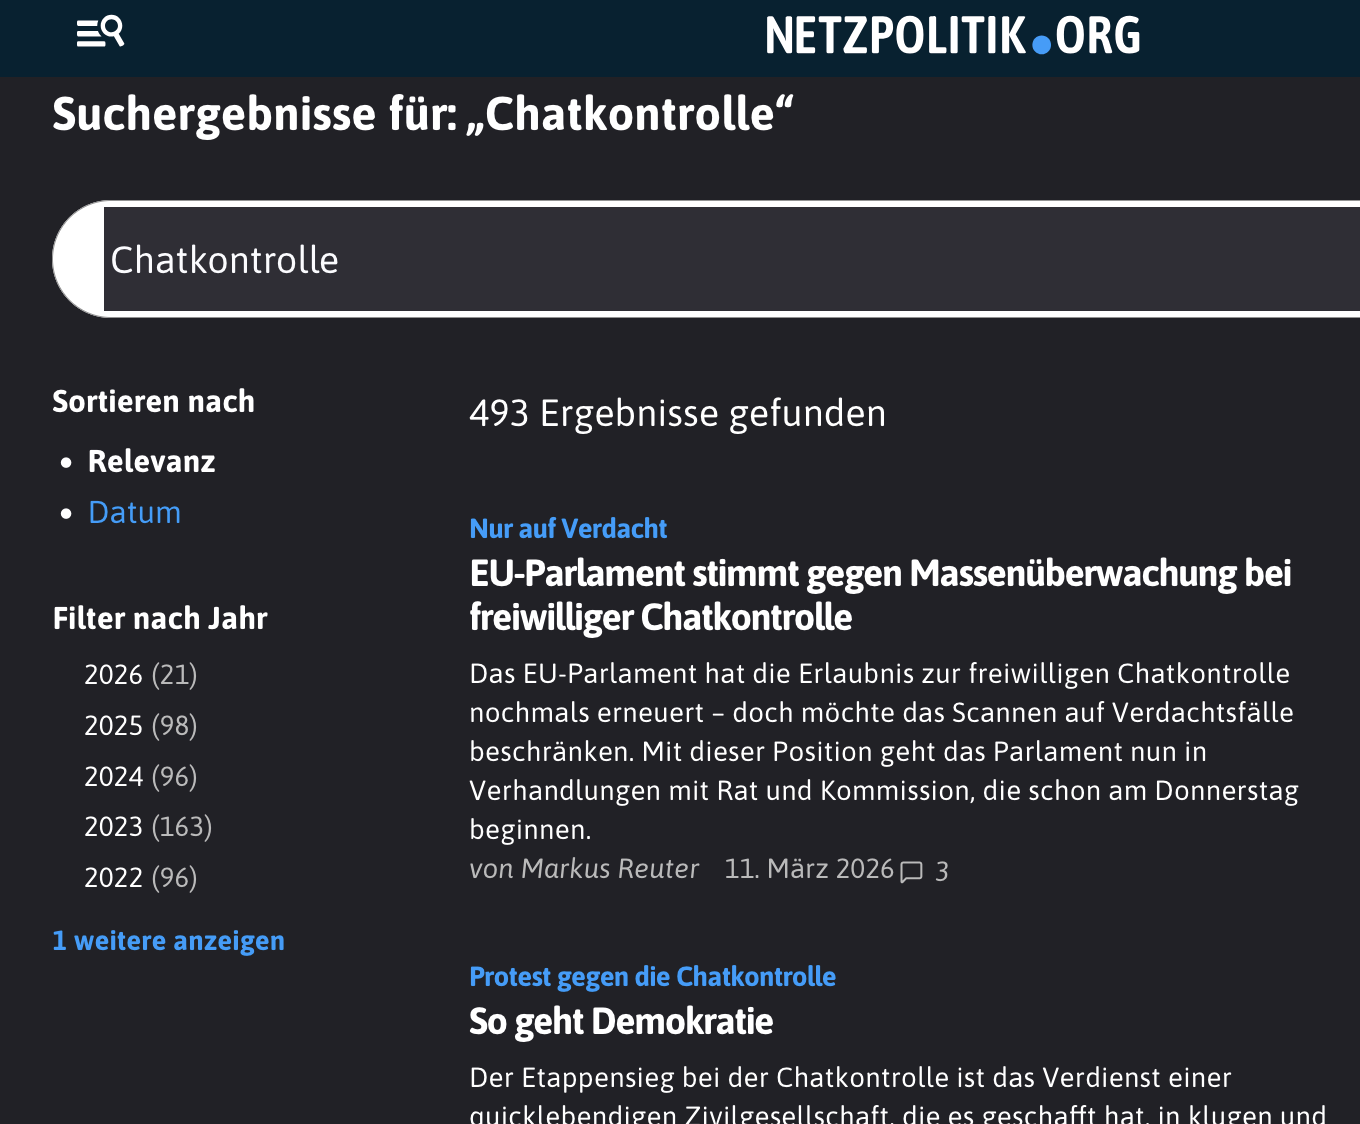
\includegraphics[keepaspectratio]{images/Screenshot 2026-06-12 at 11.23.50.png}}

}

\caption{Screenshot der ersten Suchergebnisse für ``Chatkontrolle'' auf
netzpolitik.org}

\end{figure}%

Erwartungsgemäß finden wir eine recht stattliche Menge an Ergebnissen.
Alle 493 Artikel manuell zu copy\&pasten, wäre kaum möglich
(automatisiert ist das hingegen kein Problem, dazu mehr im
Advanced-Teil). Deshalb beschränken wir uns zunächst auf die ersten 20
Artikel. Je nach Fragestellung kann es aber auch sinnvoll sein, zunächst
z.B. anhand der Überschriften nach den einschlägigsten Artikeln zu
suchen und darauf aufbauend eine Auswahl zu treffen.

Um mit den Texten korpuslinguistisch weiterarbeiten zu können, ist es
sinnvoll, sie zunächst offline zu speichern. Das geht beispielsweise,
indem man sie in ein Textdokument kopiert. Ich empfehle, hier mit einem
Texteditor wie Notepad++ oder BBEdit zu arbeiten und die Texte im
Rohtextformat .txt zu speichern. Grundsätzlich wäre es zwar auch
möglich, Texte z.B. in Word zu kopieren und dort damit weiterzuarbeiten,
aber das Rohtextformat bringt für die weitere Verarbeitung eine Reihe
von Vorteilen mit sich, während Word automatische Formatierungen usw.
anwendet, die für die weitere Prozessierung der Daten hinderlich sein
können.

Kopieren und einfügen ist denkbar einfach, vor allem, wenn man die
entsprechenden Tastenkombinationen kennt: Steuerung + C fürs Kopieren,
Steuerung + C fürs Einfügen (bei Mac: Command + C bzw. Command + V).
Figure~\ref{fig-netzpolitik01} zeigt, wie das geht.

\begin{figure}

\centering{

\pandocbounded{\includegraphics[keepaspectratio]{images/netzpolitik01.gif}}

}

\caption{\label{fig-netzpolitik01}Text in Texteditor kopieren}

\end{figure}%

Mit Strg+S können wir die Datei dann speichern. Am besten legen wir alle
Dateien in einem Ordner ab. Anschließend bietet es sich an, den Text
manuell nachzubearbeiten: Wenn wir mit Strg+A alles ausgewählt und in
eine Textdatei kopiert haben, ist darin oft auch viel sog.
Boilerplate-Text enthalten. Boilerplate-Text ist Text, der auf jeder
Seite erscheint - etwa das, was wir in Figure~\ref{fig-netzpolitik01}
nach dem Einfügen in den Texteditor ganz unten sehen:

\begin{quote}
Unterstützen

Spenden ❤️\\
Spendenservice\\
Merch-Shop

Die von uns verfassten Inhalte stehen, soweit nicht anders vermerkt,
unter der Lizenz Creative Commons BY-NC-SA 4.0.
\end{quote}

Zudem ist es im Sinne der Reproduzierbarkeit (d.h. andere Forschende
sollen in die Lage versetzt werden, unsere Forschung nachzuvollziehen
und zu überprüfen) wichtig, den Prozess der Korpuserstellung möglichst
gut zu dokumentieren. Daher ist es sinnvoll, \textbf{Metadaten} zu den
einzelnen Texten zu dokumentieren. Das kann beispielsweise in einem
eigenen Spreadsheet erfolgen -- was auch den Vorteil hat, dass wir
dieses Spreadsheet anschließend problemlos veröffentlichen können, auch
wenn wir vielleicht die Korpustexte selbst aus urheberrechtlichen
Gründen nicht weitergeben sollen. Das Sheet könnte dann etwa so
aussehen:

\begin{longtable}[]{@{}
  >{\raggedright\arraybackslash}p{(\linewidth - 8\tabcolsep) * \real{0.0939}}
  >{\raggedright\arraybackslash}p{(\linewidth - 8\tabcolsep) * \real{0.3755}}
  >{\raggedright\arraybackslash}p{(\linewidth - 8\tabcolsep) * \real{0.2708}}
  >{\raggedright\arraybackslash}p{(\linewidth - 8\tabcolsep) * \real{0.1047}}
  >{\raggedright\arraybackslash}p{(\linewidth - 8\tabcolsep) * \real{0.1552}}@{}}
\toprule\noalign{}
\begin{minipage}[b]{\linewidth}\raggedright
Dateiname
\end{minipage} & \begin{minipage}[b]{\linewidth}\raggedright
Link
\end{minipage} & \begin{minipage}[b]{\linewidth}\raggedright
Titel
\end{minipage} & \begin{minipage}[b]{\linewidth}\raggedright
Datum
\end{minipage} & \begin{minipage}[b]{\linewidth}\raggedright
Autor
\end{minipage} \\
\midrule\noalign{}
\endhead
\bottomrule\noalign{}
\endlastfoot
2025\_11\_05\_diplomaten.txt &
https://netzpolitik.org/2025/drahtbericht-deutsche-diplomaten-fordern-undiplomatisch-chatkontrolle/
& Drahtbericht: Deutsche Diplomaten fordern undiplomatisch Chatkontrolle
& 05. November 2025, 18:44 Uhr & Andre Meister \\
2025\_11\_28-faq.txt &
https://netzpolitik.org/2025/faq-wie-geht-es-weiter-mit-der-chatkontrolle/
& FAQ: Wie geht es weiter mit der Chatkontrolle? & 28. November 2025,
17:10 Uhr & Andre Meister, Anna Biselli, Markus Reuter \\
2025\_10\_04\_fragen.txt &
https://netzpolitik.org/2025/fragen-und-antworten-warum-ist-chatkontrolle-so-gefaehrlich-fuer-uns-alle/
& Fragen und Antworten : Warum ist Chatkontrolle so gefährlich für uns
alle? & 04. Oktober 2025, 12:16 Uhr & Markus Reuter \\
\ldots{} & \ldots{} & \ldots{} & \ldots{} & \ldots{} \\
\end{longtable}

Für unsere Forschungsfrage -- welche konzeptuellen Metaphern werden in
Zusammenhang mit der Chatkontrolle verwendet? -- ist es nun wichtig, die
entsprechenden Metaphern im Text zu identifizieren. Konzeptuelle
Metaphern sind Übertragungen von einer (oft konkreten) Quelldomäne auf
eine (oft abstrakte) Zieldomäne, etwa ZEIT IST RAUM: \emph{ein Treffen
nach hinten verschieben, Weihnachten naht}. Metaphern sind in der
Alltagssprache allgegenwärtig. Für die Operationalisierung unserer
Forschungsfrage ist es daher wichtig, zunächst zu entscheiden, welche
Metaphern wir identifizieren und annotieren möchten. Alle Metaphern in
unseren Texten einzubeziehen, wäre wenig zielführend, da wir ja
spezifisch herausfinden wollen, wie das Konzept ``Chatkontrolle''
metaphorisch konzeptualisiert wird (denkbare Konzeptualisierungen wären
so etwas wie \texttt{Einfallstor} für staatliche Überwachung oder
\texttt{tickende\ Zeitbombe} einerseits, \texttt{Schutzwall} gegen
Kindesmissbrauch andererseits). Daher scheint es sinnvoll, sich auf
solche Fälle metaphorischen Sprachgebrauchs zu konzentrieren, bei denen
``Chatkontrolle'' oder zumindest ein unmittelbar damit verbundenes
Konzept die Zieldomäne darstellt.

Die Identifikation von Metaphern ist alles andere als trivial,
allerdings kann man sich hier auf umfangreiche schon existierende
Forschung stützen. In der Metaphernforschung besonders etabliert zur
Identifikation von Metaphern in korpuslinguistischen Kontexten ist das
MIPVU-Verfahren, das folgende Schritte vorsieht Steen et al. (2010):

\begin{quote}
\begin{enumerate}
\def\labelenumi{\arabic{enumi}.}
\tightlist
\item
  Read the text to get a general understanding of the meaning
\item
  Determine the lexical units
\item
  a. Establish the contextual meaning of the unit b. Determine if it has
  a more basic meaning. Does the contextual meaning contrast with the
  basic meaning but can it be understood in comparison with it?
\item
  If yes, mark the unit as metaphorical.
\end{enumerate}
\end{quote}

Wir können das Verfahren nun auf einen Beispieltext anwenden, von dem
hier nur ein kurzer Ausschnitt zitiert wird:

\begin{quote}
„Wir brauchen einen Ansatz, der Grundrechte schützt statt sie
auszuhebeln``, sagt Anja Hoffmann, CEP-Datenschutzexpertin und
Ko-Autorin des Papiers. Mit dem hat sich das CEP an der EU-Konsultation
beteiligt. Ansätze wie Hintertüren, also spezielle Zugänge für
Ermittlungsbehörden zu verschlüsselten Inhalten, seien ungeeignet, führt
das Papier aus.
\end{quote}

Wir sehen, dass das Verb \emph{aushebeln} hier nicht in der
grundlegenderen Bedeutung ``mit einem Werkzeug, einem Hebel, in die Höhe
bewegen und aus einer Verankerung, einem festen Standort lösen''
(\href{https://www.dwds.de/wb/aushebeln}{DWDS}), verwendet wird.
Vielmehr wird hier die Chatkontrolle, die nicht explizit erwähnt wird,
von der wir aber aus dem weiteren Kontext erschließen können, dass sie
gemeint ist, als Werkzeug konzeptualisiert, mit dem Grundrechte, die
ihrerseits als physisches (Sicherungs-)Objekt metaphorisch dargestellt
werden, teilweise außer Kraft gesetzt oder zumindest gefährdet werden.
Auch das Wort \emph{Hintertür} wird hier offenkundig metaphorisch
verwendet und verweist auf die Konzeptualisierung des digitalen Raums
als physischen Raum.

\begin{figure}

\centering{

\pandocbounded{\includegraphics[keepaspectratio]{images/metaphernannotation_excel.gif}}

}

\caption{\label{fig-spreadsheet}Erstellung einer einfachen
Annotationstabelle mit den relevanten Textausschnitten}

\end{figure}%

Es bietet sich an, die entsprechenden Textausschnitte und die
dazugehörigen Annotationen in einem Spreadsheet zu sammeln.
Figure~\ref{fig-spreadsheet} zeigt beispielhaft, wie die relevanten
Textausschnitte aus einem Texteditor in ein Tabellenkalkulationsprogramm
wie Microsoft Excel oder LibreOffice Calc kopiert und mit weiteren
Annotationen versehen werden können. Die weiteren Annotationen stehen
dabei jeweils in einer eigenen Spalte; die am Ende entstehende Tabelle
sieht dann so aus:

\begin{longtable}[]{@{}
  >{\raggedright\arraybackslash}p{(\linewidth - 8\tabcolsep) * \real{0.0909}}
  >{\raggedright\arraybackslash}p{(\linewidth - 8\tabcolsep) * \real{0.4011}}
  >{\raggedright\arraybackslash}p{(\linewidth - 8\tabcolsep) * \real{0.2353}}
  >{\raggedright\arraybackslash}p{(\linewidth - 8\tabcolsep) * \real{0.2193}}
  >{\raggedright\arraybackslash}p{(\linewidth - 8\tabcolsep) * \real{0.0535}}@{}}
\caption{Beispieltabelle}\tabularnewline
\toprule\noalign{}
\begin{minipage}[b]{\linewidth}\raggedright
Datei
\end{minipage} & \begin{minipage}[b]{\linewidth}\raggedright
Textstelle
\end{minipage} & \begin{minipage}[b]{\linewidth}\raggedright
Metapher
\end{minipage} & \begin{minipage}[b]{\linewidth}\raggedright
metapher-evozierende sprachliche Einheit
\end{minipage} & \begin{minipage}[b]{\linewidth}\raggedright
Kommentar
\end{minipage} \\
\midrule\noalign{}
\endfirsthead
\toprule\noalign{}
\begin{minipage}[b]{\linewidth}\raggedright
Datei
\end{minipage} & \begin{minipage}[b]{\linewidth}\raggedright
Textstelle
\end{minipage} & \begin{minipage}[b]{\linewidth}\raggedright
Metapher
\end{minipage} & \begin{minipage}[b]{\linewidth}\raggedright
metapher-evozierende sprachliche Einheit
\end{minipage} & \begin{minipage}[b]{\linewidth}\raggedright
Kommentar
\end{minipage} \\
\midrule\noalign{}
\endhead
\bottomrule\noalign{}
\endlastfoot
Q5lyDSrzId-xE4nh & „Wir brauchen einen Ansatz, der Grundrechte schützt
statt sie auszuhebeln`` & Grundrechte als physisches Sicherungsobjekt &
aushebeln & NA \\
Q5lyDSrzId-xE4nh & „Wir brauchen einen Ansatz, der Grundrechte schützt
statt sie auszuhebeln`` & Chatkontrolle als Werkzeug & aushebeln & NA \\
Q5lyDSrzId-xE4nh & Hintertüren & digitaler Raum als physischer Raum &
Hintertür & NA \\
\end{longtable}

Das ist natürlich nur eine von vielen Möglichkeiten für eine sinnvolle
Herangehensweise. Wie Sie sehen, enthält die Tabelle folgende
Informationen:

\begin{itemize}
\item
  Datei: Diese Information ist wichtig, damit Sie die Textstelle der
  Datei zuordnen können, aus der sie ursprünglich stammt -- insbesondere
  dann, wenn Sie ggf. später noch einmal den weiteren Kontext
  konsultieren müssen.
\item
  Textstelle: Die relevante Textstelle (wo relevant, mit Kontext).
\item
  Metapher: Die jeweilige Metapher im Format ``Zieldomäne als
  Quelldomäne'' (alternativ könnte man auch auf die in der konzeptuellen
  Metapherntheorie gängige Schreibwiese ZIELDOMÄNE IST QUELLDOMÄNE
  zurückgreifen)
\item
  metapherevozierende sprachliche Einheit: hier wird das Lemma (also die
  Grundform) der sprachlichen Einheit vermerkt, durch die die Metapher
  evoziert wird. In den Beispielen hier sind das Verben und Substantive,
  in einigen Fällen können es aber auch andere, auch größere Einheiten
  wie idiomatische Wendungen etc. sein
\item
  Kommentar: Erfahrungsgemäß ist es oft sinnvoll, eine Kommentarspalte
  zu haben, in der besondere Beobachtungen, Zweifelsfälle, Unklarheiten
  etc. vermerkt werden können -- insbesondere dann, wenn die Annotation
  noch ``work in progress'' ist und noch nicht alle
  Annotationsentscheidungen final getroffen worden sind, denn dann kann
  man später noch einmal als unklar markierte Fälle auf Konsistenz
  überprpüfen.
\end{itemize}

Wenn man eine ausreichende Zahl an Metaphern findet, kann man auch eine
kleine quantitative Auswertung vornehmen -- weiterführende Hinweise dazu
finden sich z.B. in
\href{https://empirical-linguistics.github.io/ems/datenaufbereitung/index.html}{diesem}
Tutorial. Zugleich bietet diese Herangehensweise eine gute Möglichkeit,
mit der so erstellten, systematisch kuratierten Liste an Metaphern
qualitativ weiterzuarbeiten. Schon aus den ganz wenigen Beispielen in
(\textbf{tab-beispieltabelle?}) lassen sich einige erste Tendenzen
entnehmen, etwa dass digitale Freiheitsrechte mit Metaphern aus dem
physischen bzw. räumlichen Bereich veranschaulicht werden und die
Chatkontrolle als Werkzeug, welches das Eindringen in sonst private
Räume ermöglicht.

Das manuelle Erstellen einer Annotationstabelle via Copy \& Paste ist
natürlich relativ aufwändig. Annotationstools wie wie in der
\hyperref[advanced]{Advanced-Sektion} vorgestellten bieten teilweise
recht niedrigschwellig die Möglichkeit zur Annotation im Kontext - die
einfachste Option für eine solche eher qualitative Datenanalyse ist
derzeit wohl \href{https://openqda.org/}{OpenQDA}, worauf ich
\hyperref[openqda]{weiter unten} noch näher eingehe.

\bookmarksetup{startatroot}

\chapter{Ein eigenes Korpus erstellen: Advanced}\label{advanced}

Die oben skizzierte Herangehensweise hat den Nachteil, dass sie viel
manuelle Arbeit erfordert. Mit einigen Grundkenntnissen im Bereich
Programmierung und vor allem
\href{https://www.regular-expressions.info/}{regulären Ausdrücken} lässt
sich jedoch vieles davon automatisieren. Im Folgenden erstellen wir
zunächst eine Link-Liste in \href{https://r-project.org/}{R} und crawlen
die einzelnen Einträge in dieser Liste dann mit Trafilatura. Im
Folgenden kann ich keinen Einstieg in R geben und verweise stattdessen
auf die Vielzahl bereits existierender Ressourcen, biete aber dennoch
hoffentlich ausreichende Erklärungen, um auch für Einsteiger:innen
transparent zu machen, was die einzelnen Codezeilen tun.

\begin{tcolorbox}[enhanced jigsaw, opacityback=0, colbacktitle=quarto-callout-tip-color!10!white, colframe=quarto-callout-tip-color-frame, left=2mm, rightrule=.15mm, title=\textcolor{quarto-callout-tip-color}{\faLightbulb}\hspace{0.5em}{Tip}, toptitle=1mm, titlerule=0mm, bottomtitle=1mm, toprule=.15mm, bottomrule=.15mm, arc=.35mm, breakable, coltitle=black, leftrule=.75mm, opacitybacktitle=0.6, colback=white]

Zum Einstieg in R gibt es viele sehr empfehlenswerte Tutorials und frei
verfügbare Bücher. Besonders empfehlenswert ist die aktuelle Einführung
von LeFoll (2026); auch die
\href{https://ladal.edu.au/}{LADAL-Tutorials} von Martin Schweinberger
eignen sich gut zum Einstieg.

\end{tcolorbox}

\subsection{Link-Liste erstellen}\label{link-liste-erstellen}

Bereits oben haben wir netzpolitik.org nach dem Schlagwort
``Chatkontrolle'' durchsucht und gesehen, dass (Stand Juni 2026) 493
Artikel gefunden werden. Jeden einzelnen dieser Artikel händisch zu
copy\&pasten, wie wir es oben getan haben, wäre sehr aufwändig und ist
glücklicherweise auch nicht nötig, denn wir können z.B. das Tool
Trafilatura Barbaresi (2021) nutzen, um auch größere Mengen an Websites
zu crawlen. Dafür brauchen wir jedoch zunächst eine Link-Liste. Die
können wir zusammenstellen, indem wir die Ergebnisse unserer Suche
nutzen.

Den Link zu jedem einzelnen der 493 Ergebnisse manuell in eine Liste zu
copy\&pasten, wäre aber ähnlich aufwendig, wie alle Texte händisch zu
kopieren. Stattdessen können wir in R ein Skript schreiben, das das für
uns übernimmt. Der folgende Code ist natürlich spezifisch für
netzpolitik.org, aber die einzelnen ``Bausteine'' lassen sich auch auf
andere Websites übertragen.

Für Anfänger:innen mag der Code auf den ersten Blick komplex und
undurchschaubar wirken, er basiert aber auf einer Reihe sehr einfacher
Beobachtungen:

\begin{itemize}
\item
  Die erste Ergebnisseite hat die URL
  https://netzpolitik.org/?s=Chatkontrolle, alle weiteren Ergebnisseiten
  haben die URL
  \texttt{https://netzpolitik.org/page/i/?s=Chatkontrolle}, wobei
  \texttt{i} für die jeweilige Seite steht (2, 3, 4 etc.).
\item
  Da es 493 Treffer gibt und pro Seite (manuell nachgezählt) 20 Treffer
  angezeigt werden, muss es 493/20 = 24.65 = aufgerundet 25
  Ergebnisseiten geben.
\item
  Ein Blick in den Quelltext zeigt, dass die Links zu den einzelnen
  Artikeln in den Ergebnissen immer folgendes Format haben:
  \texttt{https://netzpolitik.org/jahr/titel}. Die Strings, die diesem
  Muster entsprechen, müssen wir also aus den Ergebnisseiten
  extrahieren. Das wird dadurch erleichtert, dass es zwar noch andere
  URLs in den Quelltexten der Ergebnisseiten gibt, bei denen jedoch
  durchweg auf \texttt{https://netzpolitik.org/} alphabetische und nicht
  numerische Zeichen folgen.
\end{itemize}

Wir müssen also zunächst die 25 Ergebnisseiten crawlen und aus diesen
Ergebnisseiten dann die Strings herausziehen, die dem Muster
\texttt{https://netzpolitik.org/}, direkt gefolgt von numerischen
Zeichen, entsprechen. Der folgende R-Code tut genau dies:

\phantomsection\label{annotated-cell-1}%
\begin{Shaded}
\begin{Highlighting}[]
\CommentTok{\# einen leere Liste erstellen}
\NormalTok{l }\OtherTok{\textless{}{-}} \FunctionTok{list}\NormalTok{()}

\CommentTok{\# über die Ergebnisliste iterieren}

\ControlFlowTok{for}\NormalTok{(i }\ControlFlowTok{in} \DecValTok{1}\SpecialCharTok{:}\DecValTok{25}\NormalTok{) \{ }\hspace*{\fill}\NormalTok{\circled{1}}
  \ControlFlowTok{if}\NormalTok{( i }\SpecialCharTok{==} \DecValTok{1}\NormalTok{) \{}
\NormalTok{    l[[i]] }\OtherTok{\textless{}{-}} \FunctionTok{readLines}\NormalTok{(}\StringTok{"https://netzpolitik.org/?s=Chatkontrolle"}\NormalTok{) }\hspace*{\fill}\NormalTok{\circled{2}}
\NormalTok{  \} }\ControlFlowTok{else}\NormalTok{ \{}
\NormalTok{    l[[i]] }\OtherTok{\textless{}{-}} \FunctionTok{readLines}\NormalTok{(}\FunctionTok{paste0}\NormalTok{(}\StringTok{"https://netzpolitik.org/page/"}\NormalTok{, }
\NormalTok{                               i,}
                               \StringTok{"/?s=Chatkontrolle"}\NormalTok{, }
                               \AttributeTok{collapse =} \StringTok{""}\NormalTok{)) }\hspace*{\fill}\NormalTok{\circled{3}}
\NormalTok{  \}}
  \FunctionTok{Sys.sleep}\NormalTok{(}\AttributeTok{time =} \FunctionTok{sample}\NormalTok{(}\DecValTok{1}\SpecialCharTok{:}\DecValTok{10}\NormalTok{, }\DecValTok{1}\NormalTok{)) }\hspace*{\fill}\NormalTok{\circled{4}}
\NormalTok{\} }

\CommentTok{\# Liste in Vektor überführen}
\NormalTok{l }\OtherTok{\textless{}{-}} \FunctionTok{unlist}\NormalTok{(l) }\hspace*{\fill}\NormalTok{\circled{5}}

\CommentTok{\# Links extrahieren}
\NormalTok{find\_links }\OtherTok{\textless{}{-}} \FunctionTok{grep}\NormalTok{(}\StringTok{"\textless{}a href=}\SpecialCharTok{\textbackslash{}"}\StringTok{https://netzpolitik.org/[0{-}9].* "}\NormalTok{, l) }\hspace*{\fill}\NormalTok{\circled{6}}
\NormalTok{l1 }\OtherTok{\textless{}{-}}\NormalTok{ l[find\_links] }\hspace*{\fill}\NormalTok{\circled{7}}

\CommentTok{\# Elemente vor und nach dem eigentlichen Link ersetzen}
\NormalTok{l1 }\OtherTok{\textless{}{-}} \FunctionTok{trimws}\NormalTok{(}\FunctionTok{gsub}\NormalTok{(}\StringTok{"\textless{}a href=}\SpecialCharTok{\textbackslash{}"}\StringTok{"}\NormalTok{, }\StringTok{""}\NormalTok{, l1)) }\hspace*{\fill}\NormalTok{\circled{8}}
\NormalTok{l1 }\OtherTok{\textless{}{-}} \FunctionTok{gsub}\NormalTok{(}\StringTok{"}\SpecialCharTok{\textbackslash{}"}\StringTok{.*"}\NormalTok{, }\StringTok{""}\NormalTok{, l1)}

\CommentTok{\# Duplikate entfernen}
\NormalTok{l1 }\OtherTok{\textless{}{-}} \FunctionTok{unique}\NormalTok{(l1) }\hspace*{\fill}\NormalTok{\circled{9}}

\CommentTok{\# Linkliste exportieren}
\FunctionTok{writeLines}\NormalTok{(l1, }\StringTok{"materialien/linkliste.txt"}\NormalTok{) }\hspace*{\fill}\NormalTok{\circled{10}}
\end{Highlighting}
\end{Shaded}

\begin{description}
\tightlist
\item[\circled{1}]
wir wissen, dass es 25 Ergebnisseiten geben muss, weil pro Seite 20
Einträge angezeigt werden und es 493 Ergebnisse gibt
\item[\circled{2}]
Ab der zweiten Ergebnisseite muss bei der URL die
\texttt{/page}-Erweiterung angegeben werden, die für die erste Seite
noch entfällt. Mit diesem if-Statement stellen wir sicher, dass die
erste Ergebnisseite entsprechend anders behandelt wird als die
folgenden.
\item[\circled{3}]
die i-te Ergebnisseite wird als i-tes Element der Liste hizugefügt.
\item[\circled{4}]
mit Sys.sleep können wir einen kurzen Abstand zwischen den Anfragen
einbauen, was bei der Abfrage von größeren Datenmengen sinnvoll sein
kann, um die Server zu schonen
\item[\circled{5}]
Dieser Befehl überführt die Liste in einen Vektor, der anschließend
weiter verarbeitet werden kann.
\item[\circled{6}]
Eine manuelle Inspektion des Quelltexts zeigt, dass alle Links mit
https://netzpolitik.org/ beginnen, gefolgt von einer Zahl - Letzterem
tragen wir mit dem regulären Ausdruck \texttt{{[}0-9{]}} Rechnung.
Dieser \texttt{grep}-Befehl sucht also alle Elemente in unserem Vektor,
in denen dieses Link-Muster zu finden ist.
\item[\circled{7}]
Hier wird das Subset unseres Vektors mit allen Elementen erstellt, die
das eben gesuchte Muster enthalten.
\item[\circled{8}]
In dieser und der folgenden Zeile werden alle Elemente vor und nach dem
eigentlichen Link gelöscht. \texttt{trimws} steht für ``trim
whitespace''; diese Funktion entfernt Leerzeichen am Anfang und am Ende
des Strings.
\item[\circled{9}]
Viele Links treten im gecrawlten Quelltext mehrfach auf, deshalb werden
sie hier dedupliziert.
\item[\circled{10}]
Dieser Befehl schließlich exportiert die Links in eine Linkliste.
\end{description}

Das Ergebnis des Codes ist die Linkliste, die im Textdokument
\texttt{linkliste.txt} gespeichert ist.

\subsection{Crawlen mit Trafilatura}\label{crawlen-mit-trafilatura}

Als nächstes können wir die Linkliste als Input für Trafilatura nutzen.
Trafilatura ist eine Python-Programmbibliothek, die man aber auch
einfach übers Terminal aufrufen kann. Es gäbe zwar auch R-Libraries, die
einen ähnlichen Zweck erfüllen, z.B. \texttt{rvest}, aber Trafilatura
hat den Vorteil, dass es viele Prozessierungsschritte automatisch
erledigt, die wir andernfalls manuell erledigen müssten (z.B. die
Entfernung von Boilerplate-Text). Wenn Trafilatura korrekt installiert
ist, genügt folgender Terminal-Befehl, um die Daten zu crawlen:

\begin{Shaded}
\begin{Highlighting}[]
\NormalTok{trafilatura {-}i materialien/linkliste.txt {-}o materialien/netzpolitik\_daten {-}{-}with{-}metadata {-}{-}formatting {-}{-}output{-}format txt}
\end{Highlighting}
\end{Shaded}

Der Befehl ist wie folgt zu lesen:

\begin{itemize}
\item
  \texttt{-i} (Input) gibt an, wo die Datei mit der Link-Liste liegt,
  die gecrawlt werden soll;
\item
  \texttt{-o} (Output) gibt an, wo die Ergebnisse gespeichert werden
  sollen;
\item
  \texttt{-\/-with-metadata} gibt an, dass die gespeicherten Dateien
  auch Metadaten enthalten sollen (z.B. Datum);
\item
  \texttt{-\/-formatting} gibt an, dass die Dateien auch Informationen
  zur Formatierung enthalten sollen (z.B. bei welchen Textstrings es
  dich um Überschriften handelt);
\item
  \texttt{-\/-output-format} gibt an, dass wir die Dateien als
  Rohtextdateien (.txt) haben möchten.
\end{itemize}

\subsection{Annotation in dezidierter
Annotationssoftware}\label{annotation-in-dezidierter-annotationssoftware}

Wärend wir im Quick\&Dirty-Ansatz noch alle relevanten Segmente manuell
aus den Daten herauskopiert haben, können wir sie dank entsprechender
Software auch in eigens für solche Zwecke entwickelter
Annotationssoftware mit Annotationen versehen. In der qualitativen
Forschung ist das kommerzielle Tool MAXQDA nach wie vor der
sprichwörtliche Platzhirsch; tatsächlich ist es von der
Benutzerfreundlichkeit und Funktionsvielfalt her das wahrscheinlich
einsteigerfreundlichste Tool, und viele Universitäten oder Institute
haben Lizenzen dafür. Inzwischen gibt es aber erfreulicherweise auch
kostenlose und quelloffene Alternativen, auf die wir uns hier
beschränken wollen.

\subsubsection{OpenQDA}\label{openqda}

Die niedrigschwelligste und einfachste Option ist derzeit wohl
\href{https://openqda.org/}{OpenQDA}, das online verwendbar und denkbar
einfach zu bedienen ist. Hier können wir zunächst ein neues Projekt
erstellen. Links sehen wir eine Sidebar, in der verschiedene Optionen
verfügbar sind; die Schritte ``Preparation'', ``Coding'' und
``Analysis'', die hier ausgewählt werden können\ldots{}

\begin{figure}[H]

{\centering \pandocbounded{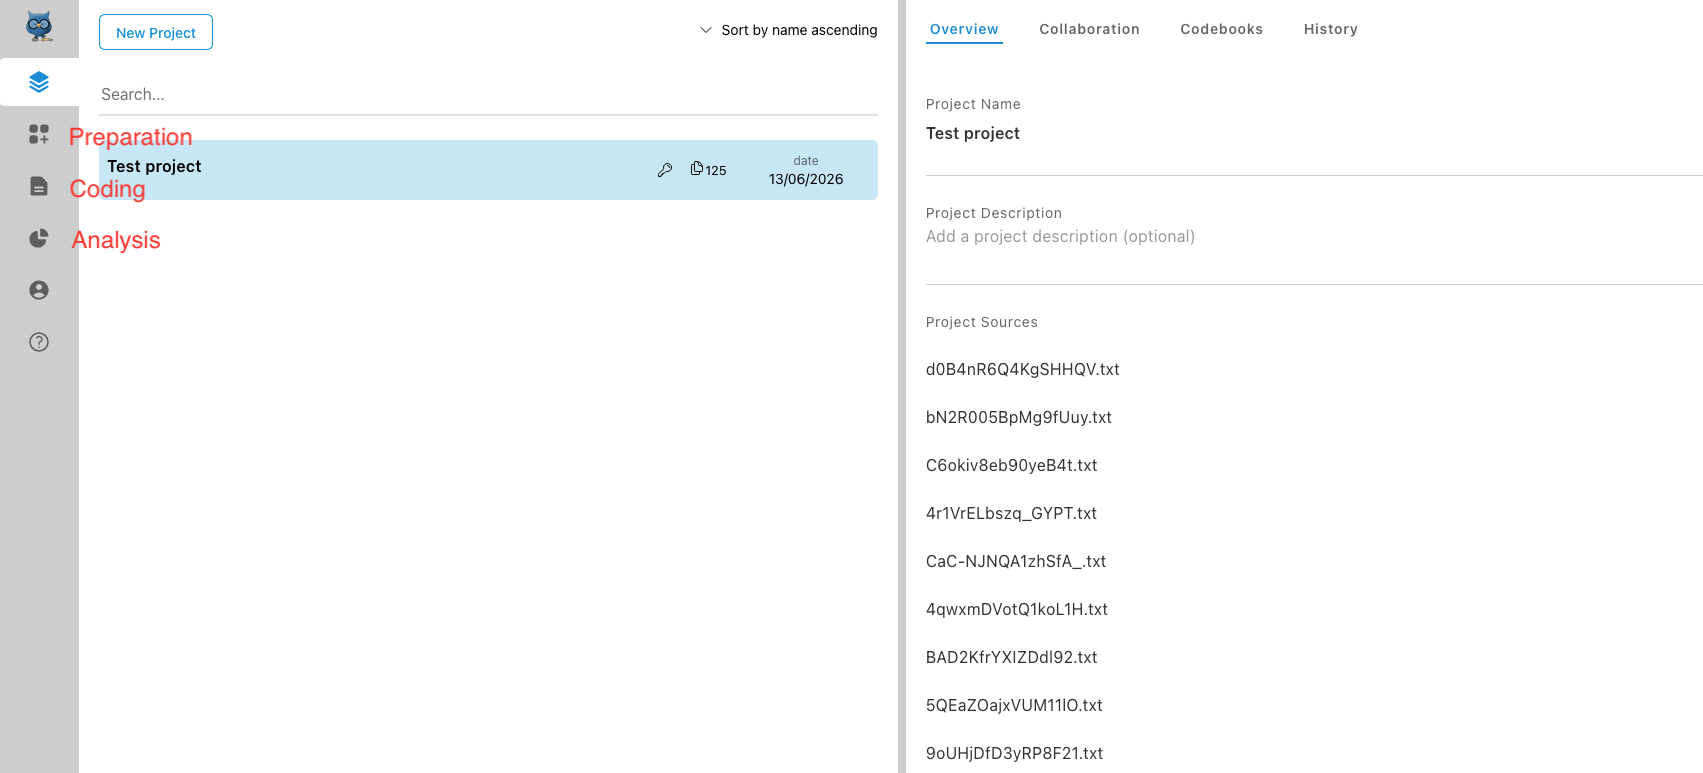
\includegraphics[keepaspectratio]{images/openqda-sidebar.png}}

}

\caption{OpenQDA-Workflow-Sidebar.}

\end{figure}%

\ldots{} müssen wir nun nacheinander abarbeiten.

Nach Import der über Trafilatura gecrawlten Dateien können wir diese im
``Preparation''-Tab theoretisch weiter bearbeiten, was wir aber an
dieser Stelle nicht wollen -- wir wollen direkt in die Kodierung
einsteigen. Um ein Dokument kodieren zu können, müssen wir es zuerst für
die weitere Textbearbeitung sperren (``Lock for Coding''), was im
Preparation-Tab geschieht:

\begin{figure}[H]

{\centering \pandocbounded{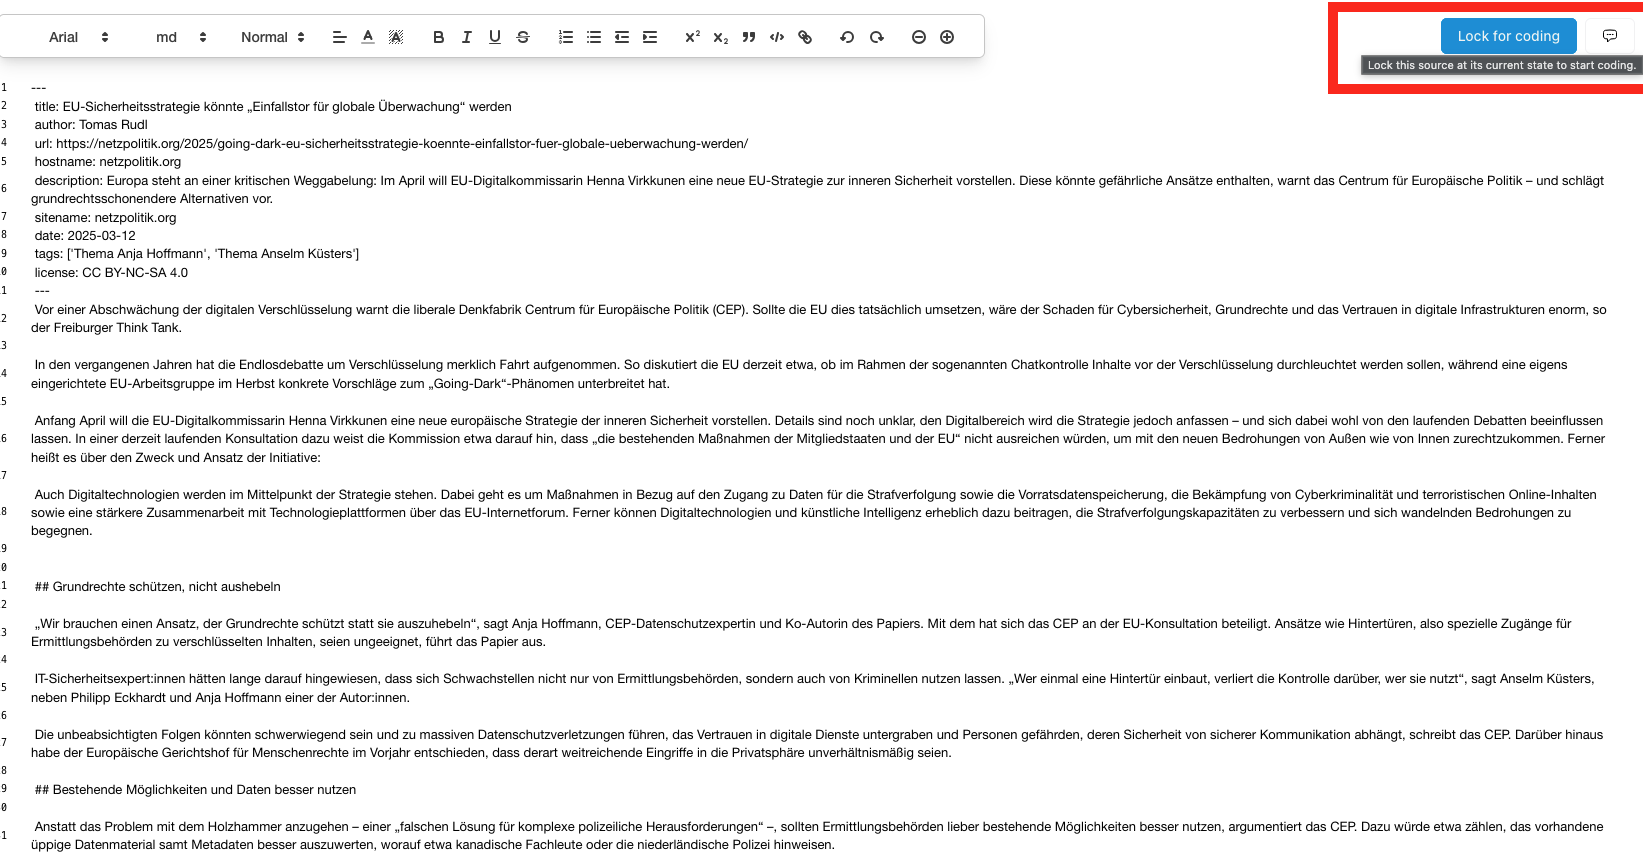
\includegraphics[keepaspectratio]{images/ openqda-lockforcoding.png}}

}

\caption{Der Lock-for-Coding-Button in OpenQDA.}

\end{figure}%

Wenn wir im Folgenden auf ``Confirm'' klicken, werden wir direkt in den
Coding-Tab weitergeleitet, wo wir das Dokument nun bearbeiten können und
wo wir links unter ``Sources'' zwischen allen Dokumenten wählen können,
die wir bereits für die Kodierung freigegeben haben (bei mir sind das im
folgenden Screenshot schon ein paar mehr).

\begin{figure}[H]

{\centering \pandocbounded{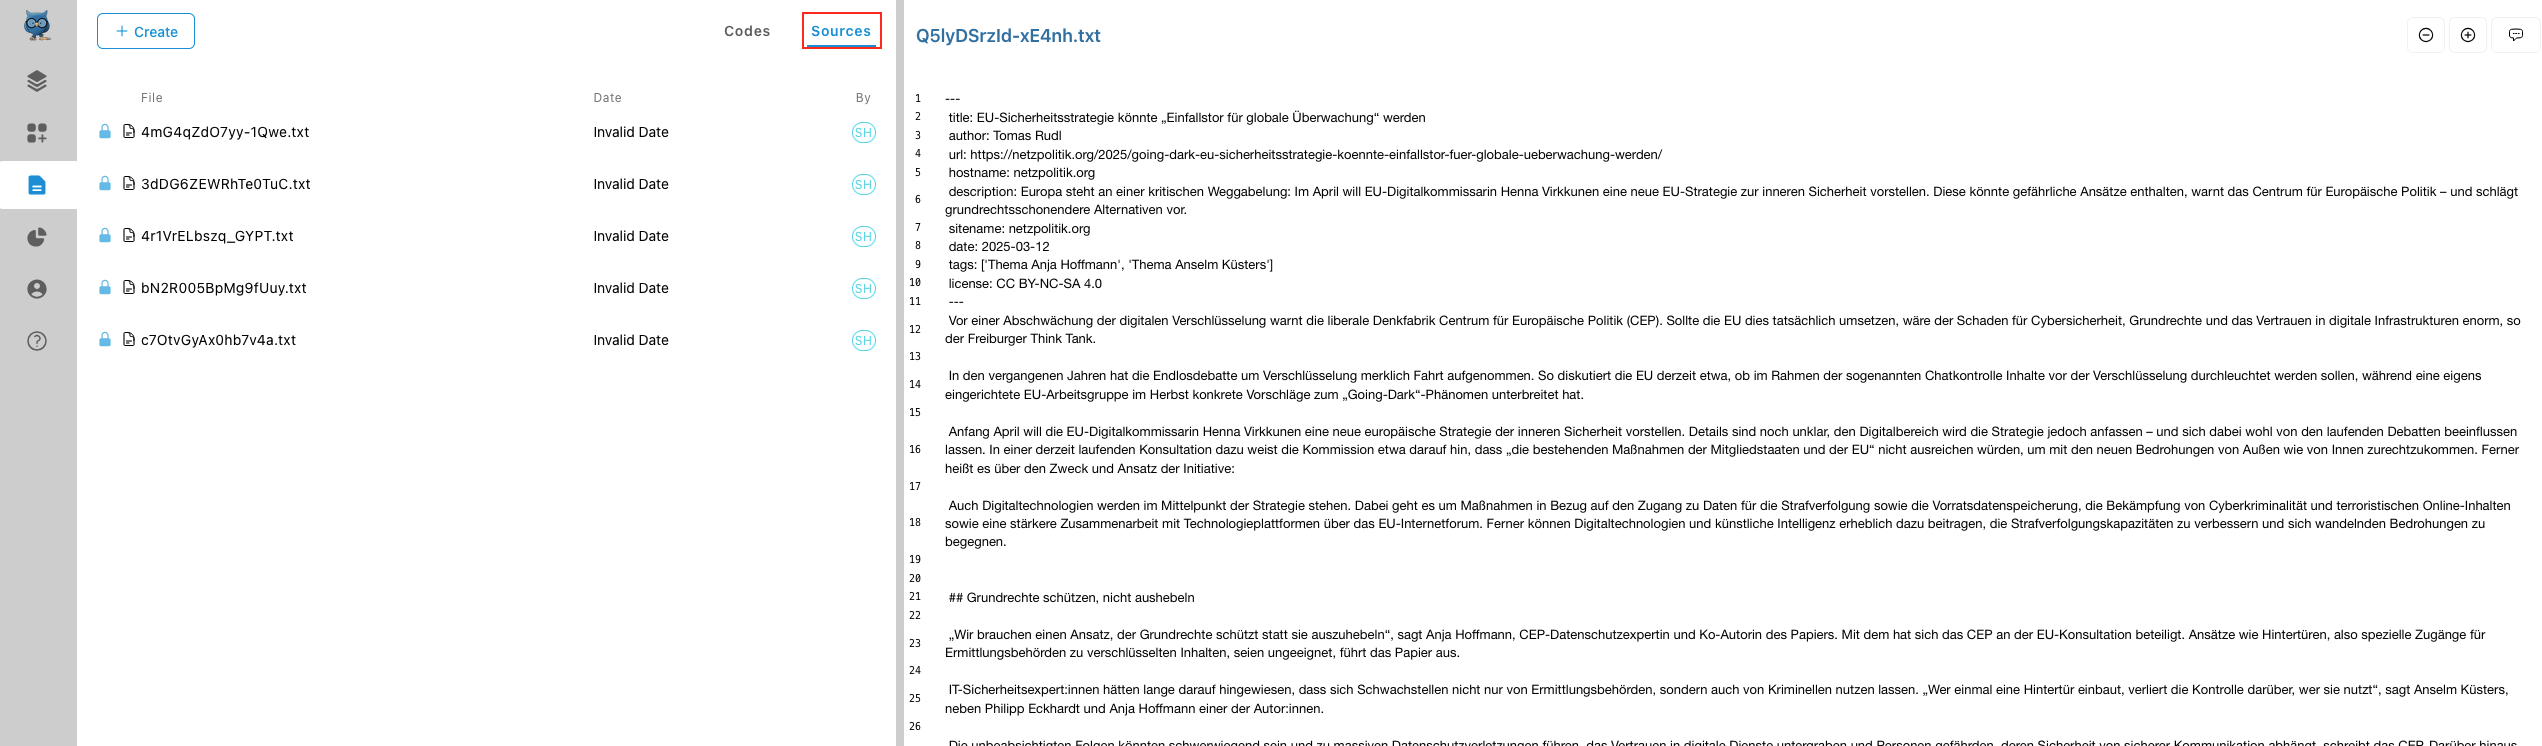
\includegraphics[keepaspectratio]{images/openqda-coding01.png}}

}

\caption{Coding-Ansicht von OpenQDA mit Sources-Auswahl}

\end{figure}%

Nun können wir erste Annotationen vornehmen, indem wir einzelne Wörter
oder Spannen im Text markieren, worauf am oberen rechten Rand ein
``Menu''-Button erscheint, auf den wir klicken können, um mit ``Create
new in-vivo-Code'' einen neuen Code zu erstellen. Einen einmal
erstellten Code können wir für andere Textsegmente auch wiederverwenden:
sobald wir einen Code erstellt haben, steht er bei weiteren Annotationen
im Auswahlmenü zur Verfügung

\begin{figure}[H]

{\centering \pandocbounded{\includegraphics[keepaspectratio]{images/openqda-annotation.gif}}

}

\caption{Beispiel für Kodierungen (Annotationen) in OpenQDA.}

\end{figure}%

Wenn wir mit den Annotationen fertig sind, können wir die annotierten
Segmente mit den Annotationen auch im CSV-Format exportieren. Dafür
müssen wir in den ``Analysis''-Tab wechseln. Die Option ``Export to
CSV'' ist zunächst ausgegraut, weil wir zuerst eine Option im
Dropdown-Menü ``Select a visualization'' wählen müssen.

\begin{figure}[H]

{\centering \pandocbounded{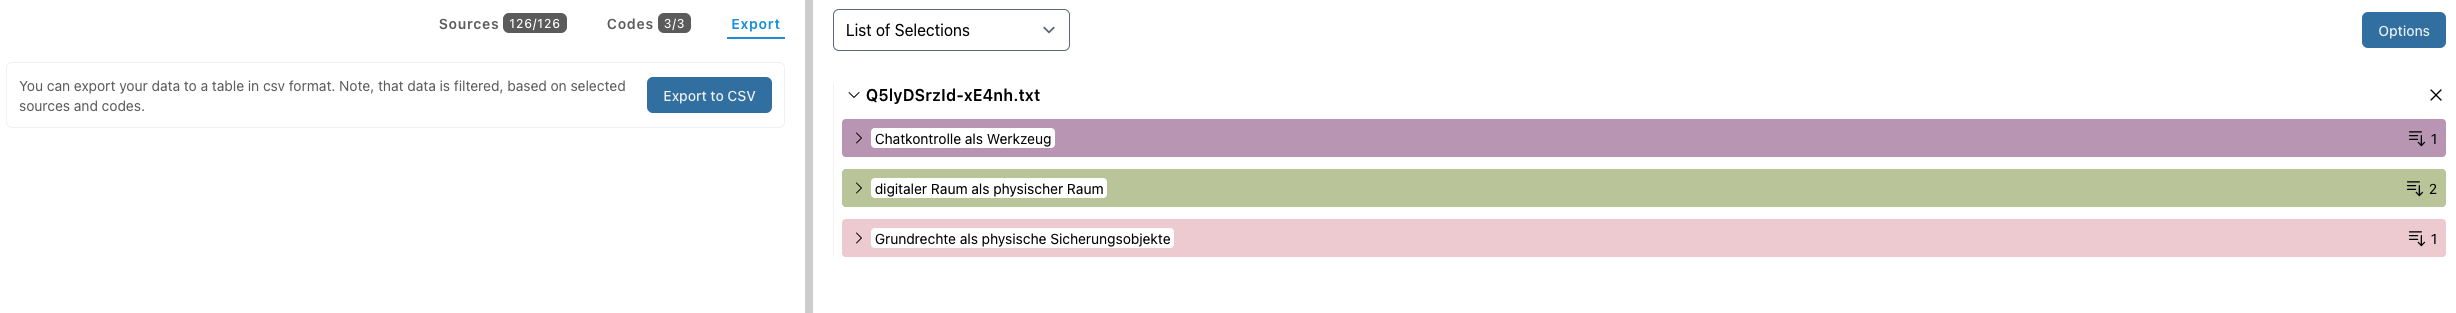
\includegraphics[keepaspectratio]{images/ openqda_csv_export.png}}

}

\caption{CSV-Export in OpenQDA}

\end{figure}%

Das resultierende Spreadsheet ist ganz ähnlich wie
Figure~\ref{fig-spreadsheet} oben, auch wenn die zusätzlichen Spalten,
die wir dort hinzufügen konnten, hier natürlich fehlen -- bei Bedarf
können wir sie noch manuell in einem Tabellenkalkulationsprogramm
ergänzen.

\begin{figure}[H]

{\centering \pandocbounded{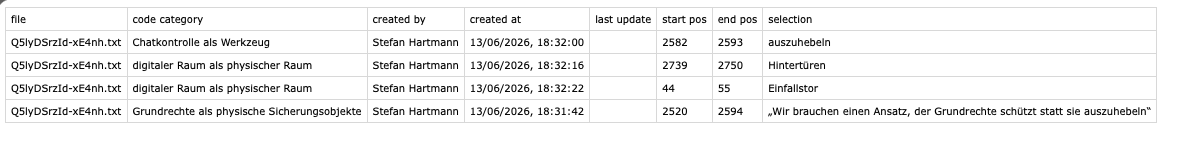
\includegraphics[keepaspectratio]{images/openqda_csv_result.png}}

}

\caption{Das Spreadsheet, das aus den oben vorgenommenen Annotationen
resultiert.}

\end{figure}%

\subsubsection{INCEpTION}\label{inception}

\href{https://inception-project.github.io/}{INCEpTION} ist ein
vielseitiges Annotationstool, das einen deutlich größeren
Funktionsumfang bietet als OpenQDA, aber auch anspruchsvoller ist. Es
ist vor allem für serverbasierte Nutzung ausgelegt, man kann es aber
auch auf dem eigenen Rechner verwenden. Sofern man Java installiert hat,
genügt es in der Regel, die auf der Website verfügbare .jar-Datei
herunterzuladen und zu öffnen. INCEpTION öffnet sich dann in Ihrem
Browser, wo Sie bei der ersten Verwendung zunächst ein Admin-Passwort
vergeben müssen.

\begin{tcolorbox}[enhanced jigsaw, opacityback=0, colbacktitle=quarto-callout-warning-color!10!white, colframe=quarto-callout-warning-color-frame, left=2mm, rightrule=.15mm, title=\textcolor{quarto-callout-warning-color}{\faExclamationTriangle}\hspace{0.5em}{Achtung!}, toptitle=1mm, titlerule=0mm, bottomtitle=1mm, toprule=.15mm, bottomrule=.15mm, arc=.35mm, breakable, coltitle=black, leftrule=.75mm, opacitybacktitle=0.6, colback=white]

Notieren Sie sich unbedingt das Admin-Passwort, das Sie vergeben. Für
die lokale Nutzung gibt es naheliegenderweise keine
Password-Reset-Option.

\end{tcolorbox}

Anschließend können wir ein neues Projekt erstellen -- hier verwenden
wir die Option ``Classic linguistic project'' (wir könnten aber auch
einfach ein ``Blank project'' erstellen). Nun können wir über die
Importfunktion die über Trafilatura gecrawlten Dateien einlesen.

\begin{tcolorbox}[enhanced jigsaw, opacityback=0, colbacktitle=quarto-callout-caution-color!10!white, colframe=quarto-callout-caution-color-frame, left=2mm, rightrule=.15mm, title=\textcolor{quarto-callout-caution-color}{\faFire}\hspace{0.5em}{Hinweis}, toptitle=1mm, titlerule=0mm, bottomtitle=1mm, toprule=.15mm, bottomrule=.15mm, arc=.35mm, breakable, coltitle=black, leftrule=.75mm, opacitybacktitle=0.6, colback=white]

Beim Einlesen der von Trafilatura gecrawlten .txt-Dateien kann es
aufgrund der Dateinamen, die Trafilatura vergibt, zu einer Fehlermeldung
kommen:

\begin{figure}[H]

{\centering \pandocbounded{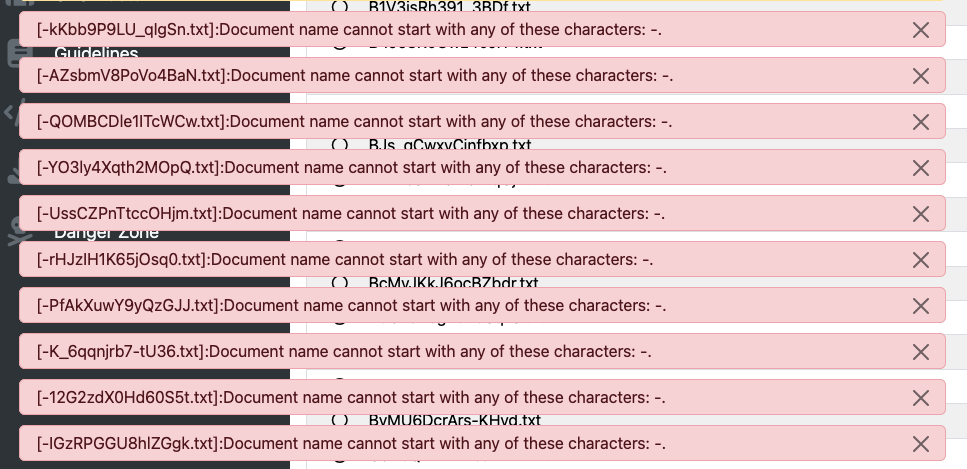
\includegraphics[keepaspectratio]{images/inception_character_error.png}}

}

\caption{Fehlermeldung in INCEpTION beim Datenimport}

\end{figure}%

Wie aus der Fehlermeldung klar hervorgeht, akzeptiert INCEpTION keine
Dateinamen, die mit \texttt{-} anfangen. Zum Glück können wir die
Dateinamen über einen einfachen Terminal-Befehl relativ schnell ändern.
(Transparenzhinweis: Die beiden Befehle wurden mit Hilfe von ChatGPT
erstellt.)

Um die Befehle anzuwenden, müssen wir zunächst mit dem
\texttt{cd}-Befehl in das entsprechende Verzeichnis navigieren.
Anschließend sollten Sie die Befehle einfach copy\&pasten und ausführen
können.

In Mac (zsh):

\begin{Shaded}
\begin{Highlighting}[]
\NormalTok{for f in {-}{-} {-}*; do}
\NormalTok{    [[ {-}e "$f" ]] || continue}
\NormalTok{    mv {-}{-} "$f" "x$f"}
\NormalTok{done}
\end{Highlighting}
\end{Shaded}

In Windows (PowerShell):

\begin{Shaded}
\begin{Highlighting}[]
\NormalTok{Get{-}ChildItem {-}File | Where{-}Object \{}
\NormalTok{    $\_.Name.StartsWith(\textquotesingle{}{-}\textquotesingle{})}
\NormalTok{\} | ForEach{-}Object \{}
\NormalTok{    Rename{-}Item {-}LiteralPath $\_.FullName {-}NewName ("x" + $\_.Name)}
\NormalTok{\}}
\end{Highlighting}
\end{Shaded}

\end{tcolorbox}

\begin{figure}[H]

{\centering \pandocbounded{\includegraphics[keepaspectratio]{images/inception_import.gif}}

}

\caption{Erstellung eines neuen Projekts und Datenimport in INCEpTION}

\end{figure}%

Bevor wir mit der Annotation loslegen können, müssen wir einen
entsprechenden Annotations-Layer kreieren. In der Sidebar links sehen
wir die Option ``Layers'' (falls Sie die Sidebar nicht sehen können: Sie
befindet sich im ``Settings''-Menü des Projekts), wo wir einen neuen
Layer anlegen können.

\begin{figure}[H]

{\centering \pandocbounded{\includegraphics[keepaspectratio]{images/inception-create-layer.gif}}

}

\caption{Erstellung eines neuen Annotations-Layers in INCEpTION}

\end{figure}%

Sobald der Layer erstellt ist, kann die eigentliche Annotation beginnen.
Dafür müssen wir zunächst auf ``Dashboard'' klicken, dann auf
``Annotation'' und ein Dokument zum Annotieren auswählen.

\begin{figure}[H]

{\centering \pandocbounded{\includegraphics[keepaspectratio]{images/inception-annotation.gif}}

}

\caption{Annotation in INCEpTION}

\end{figure}%

\subsection{Lemmatisierung und
POS-Tagging}\label{lemmatisierung-und-pos-tagging}

Optional können wir die Daten nun auch noch lemmatisieren und mit
POS-Tags versehen. Dafür nutzen wir die
\href{https://spacyr.quanteda.io/}{\texttt{spacyr}}-Programmbibliothek.

\phantomsection\label{annotated-cell-3}%
\begin{Shaded}
\begin{Highlighting}[]
\FunctionTok{library}\NormalTok{(tidyverse) }\hspace*{\fill}\NormalTok{\circled{1}}
\FunctionTok{library}\NormalTok{(spacyr) }\hspace*{\fill}\NormalTok{\circled{2}}
\FunctionTok{library}\NormalTok{(udpipe) }\hspace*{\fill}\NormalTok{\circled{3}}

\CommentTok{\# Liste aller Dateien}
\NormalTok{f }\OtherTok{\textless{}{-}} \FunctionTok{list.files}\NormalTok{(}\StringTok{"materialien/netzpolitik\_daten/"}\NormalTok{, }\AttributeTok{full.names =} \ConstantTok{TRUE}\NormalTok{) }\hspace*{\fill}\NormalTok{\circled{4}}

\CommentTok{\# Datei einlesen}
\NormalTok{d }\OtherTok{\textless{}{-}} \FunctionTok{readLines}\NormalTok{(f[}\DecValTok{1}\NormalTok{])}

\CommentTok{\# Header auslesen}
\NormalTok{hdr }\OtherTok{\textless{}{-}} \FunctionTok{grep}\NormalTok{(}\StringTok{"{-}{-}{-}"}\NormalTok{, d[}\DecValTok{1}\SpecialCharTok{:}\DecValTok{20}\NormalTok{]) }\hspace*{\fill}\NormalTok{\circled{5}}

\CommentTok{\# separate\_wider\_delim(d[(hdr[1]+1):(hdr[2]{-}1)])}
\end{Highlighting}
\end{Shaded}

\begin{description}
\tightlist
\item[\circled{1}]
brauchen wir für einige der unten angewandten Funktionen, u.a. die
\texttt{separate\_wider\_delim}-Funktion
\item[\circled{2}]
brauchen wir für Lemmatisierung und POS-Tagging
\item[\circled{3}]
brauchen wir für den Export im CoNNL-U-Format.
\item[\circled{4}]
erstellt eine Liste mit den Dateien, die im nächsten Schritt eingelesen
werden.
\item[\circled{5}]
Mit `---` wird in den Trafilatura-Ergebnisdateien der Header mit
Metadaten abgegrenzt. Für den unwahrscheinlichen Fall, dass irgendwo im
Text noch der String `---` vorkommt, durchsuchen wir nur die ersten 20
Zeilen.
\end{description}

\bookmarksetup{startatroot}

\chapter*{References}\label{references}
\addcontentsline{toc}{chapter}{References}

\markboth{References}{References}

\phantomsection\label{refs}
\begin{CSLReferences}{1}{0}
\bibitem[\citeproctext]{ref-barbaresi2021}
Barbaresi, Adrien. 2021. {``Trafilatura: A Web Scraping Library and
Command-Line Tool for Text Discovery and Extraction.''} In.

\bibitem[\citeproctext]{ref-lefoll2026}
LeFoll, Elen. 2026. \emph{Data Analysis for the Language Sciences. {A}
Very Gentle Introduction to Statistics and Data Visualization in {R}}.
\url{https://elenlefoll.github.io/RstatsTextbook/}.

\bibitem[\citeproctext]{ref-luth2022}
Luth, Janine, Konstanze Marx, and Christian Pentzold. 2022. {``Ethische
Und Rechtliche Aspekte Der Analyse von Digitalen Diskursen.''} In,
edited by Eva Gredel, 99--134. Berlin, Boston: De Gruyter.
\url{https://doi.org/10.1515/9783110721447-006}.

\bibitem[\citeproctext]{ref-steenMethodLinguisticMetaphor2010}
Steen, Gerard, Aletta G. Dorst, J. Berenike Herrmann, Anna A. Kaal, Tina
Krennmayr, and Trijntje Pasma. 2010. \emph{A Method for Linguistic
Metaphor Identification: From {MIP} to {MIPVU}}. Converging Evidence in
Language and Communication Research 14. Amsterdam, Philadelphia: John
Benjamins.

\end{CSLReferences}




\end{document}
